%%%%%%%%%%%%%%%%%%%%%%%%%%%%%%%%%%%%%%%%%%%%%%
% Header
\documentclass[11pt]{report}
\usepackage[english]{babel}
\usepackage[utf8x]{inputenc}
\usepackage{hyperref}
\usepackage{graphicx}
\usepackage{fullpage}
\usepackage{enumitem}
\usepackage{color,soul}
\usepackage[lastexercise]{exercise}

\setlength{\parindent}{0cm}

\renewcommand{\ExerciseName}{Part}

\renewcommand{\ExerciseHeader}{\large\textbf{\ExerciseName~\ExerciseHeaderNB} - \textbf{\ExerciseTitle}\medskip}

\renewcommand{\ExePartHeader}{\medskip\textbf{\ExePartName\ExePartHeaderNB\ExePartHeaderTitle\medskip}}

\begin{document}
%%%%%%%%%%%%%%%%%%%%%%%%%%%%%%%%%%%%%%%%%%%%%%
\title{Assignment 1: Small Project - Building Programs}
\subsubsection*{EMAT10007 -- Introduction to Computer Programming}
\subsection*{\Large Assignment 2020 -- Encrypted Information}

\section*{Overview}
\begin{itemize}
	\item The objective of the assignment is to submit an interactive Python program that allows the user to:
	\begin{itemize}
		\item Encrypt/decrypt messages using a Caesar cipher.
		\item Input the message to be encrypted/decrypted.
		\item Specify the rotation used by the Caesar cipher.
		\item Extract statistics about the messages, such as letter frequency, average word length, etc.
		\item Extract, manipulate and create a visual representation of information contained in a decrypted message 
% 		\item To automate the identification of the rotation used by some encrypted message.
	\end{itemize}
	\item Your Python program should be accompanied by a {\bf short, 1-2 page} report. This should discuss your implementation and any design choices. For example, why you chose to use a specific data structure or how you improved the reusability of your code. 
 	\item \textbf{The \textbf{deadline is 15:00 on Friday 11th Decemeber}} You must upload your assignment including the program (.py), report (.PDF) and any output files generated by the program (.csv, .pdf) to \textbf{Blackboard}.
	\item You must show which part of the assignment each section of your code answers by adding comments showing part and sub-section (e.g. Part 1.1) using the following format :

    \vspace{0.5em}
    {\tt \#\ PART 1.1 Comment here ...}
    \vspace{0.5em}
    
    Note that the order that the answers to the questions appear in the code may be different to the order they appear in this document so it is important to indicate to the marker where you have attempted to answer each question. You should also use comments to show what your code does. 
    \item This is an individual project. You may discuss the creative approaches to solve your assignment with each other, but you must work individually on all of the programming. 
    	\textbf{We will be checking for plagiarism!}
    \end{itemize}
    
\vspace{1em}
\hrule
\vspace{1em}
    
    \subsection*{Helpful hints and suggestions}
\begin{itemize}
    \item Complete all of the exercise sheets first - they have been designed to prepare you for this assignment.
	\item You should spend plenty of time planning the flow of your program \textbf{before} you start programming. Look back at previous exercise sheets to see how to approach larger problems by breaking them down into smaller ones.
	\item Remember to think about the \textbf{readability} and \textbf{reusability} of your code. Some question you should ask yourself:
	\begin{itemize}
		\item Have I named things sensibly? Could someone pick up my code and understand it?
		\item Am I repeating lots of code? Can I reuse any?
		\item Can I simplify the layout of my code to make it more readable? 
	\end{itemize}
% 	\item \textbf{Comment your code!} Comments are crucial for many reasons:
% 	\begin{itemize}
% 		\item They help other readers to understand what your code is doing.
% 		\item They help \emph{you} remember what your code is doing, when you come back to it weeks/months/years later. The whole point of writing code is that it can be reused many times, so to make it reusable, add comments.
% 		\item To help your TA assess your understanding of the problem you are trying to solve, and to assess how well your solution solves it. If you use a data structure to implement some functionality, explain it in the comments.
% 	\end{itemize}
% 	Short comments are great to summarise the next several lines of code by giving a high-level overview. For longer, more detailed comments (likely useful in functions and for Part 4), by enclosing them in three speech marks {\tt """} either side. E.g.
	
% 	\vspace{0.5em}
% 	{\tt def SomeFunction(SomeArgument):}\\
% 	{\tt \hspace*{2em}"""}\\
% 	{\tt \hspace*{2em}This function does ...}\\
% 	{\tt \hspace*{2em}....and it does this....}\\
% 	{\tt \hspace*{2em}"""}
% 	\vspace{0.5em}
	
	\item You will gain marks for: % mark for the following points:
	\begin{itemize}
	    %\item Functionality: Does your program do what it is supposed to. %The more of the functionality described above you implement, the higher the mark.
	    \item Types: Proper use of data types and data structures. 
	    \item Comments: Appropriate and useful comments. 
	    \item Naming: Appropriate variable and function names (remember we want you to use CamelCase)
	    \item Report: Informative report, which explains your thought process and analyses the choices you made in your code design. You must reference any external code or ideas used.
	    \item Working code: Does the code do what it is supposed to? {\bf READ THE QUESTIONS CAREFULLY to check}. Is the program robust, i.e., does it deal correctly with wrong inputs (user/program interaction).
	\end{itemize}
	
	\item Finally, don't forget to ask for help! You will be able to ask your TA for help and advice during the weekly drop-in sessions and tutorials. 
\end{itemize}

    
\newpage

\section*{Background: The basics of cryptography}
\begin{itemize}
	\item A \href{https://en.wikipedia.org/wiki/Caesar_cipher}{Caesar cipher} is a simple, well known cipher used in the encryption of strings. It is a `substitution cipher', meaning that each letter is \emph{substituted} with a corresponding letter in the alphabet at a predefined offset from the input letter's position. The the size of the offset is called the \emph{rotation}.\\
	\item The table below shows a Caesar cipher with a rotation value of $13$; a popular special case of the Caesar cipher known as \href{https://www.wikiwand.com/en/ROT13}{ROT13}.
	\begin{table}[h]
		\centering
		\begin{tabular}{|r|c|c|c|c|c|c|c|c|c|c|c|c|c|c|c|c|}
		\hline
		\textbf{Index} & {\tt 0} & {\tt 1} & {\tt 2} & {\tt 3} & {\tt 4} & {\tt 5} & {\tt 6} & {\tt 7} & {\tt 8} & {\tt 9} & {\tt 10} & {\tt 11} & {\tt 12} & 13 & ... \\ \hline
		\textbf{Input} & A & B & C & D & E & F & G & H & I & J & K  & L  & M & N & ... \\ \hline
		\textbf{Output} & N & O & P & Q & R & S & T & U & V & W & X  & Y  & Z & A & ... \\ \hline
		\end{tabular}
	\end{table}
	\item In this example, the letter ``A'' is replaced by the letter indexed $13$ positions to the right of ``A''; the letter ``N''.
	\item This particular cipher is only defined for the letters of the alphabet, meaning that punctuation, spaces, and numbers are left unchanged.
\end{itemize}

\newpage

\begin{Exercise}[title=Encryption and Decryption]
	\Question{Your program should ask the user for the following information:
	\begin{itemize}
		\item The {\tt cipher mode} : encrypt or decrypt the message
% 		\begin{itemize}
% 		    \item Should it {\tt encrypt} or {\tt decrypt} the message?
% 		\end{itemize}
		\item A {\tt rotation value} : how many places should the cipher shift each character. 
% 		\begin{itemize}
% 		    \item How far should the cipher shift?
% 		    \item This should be a positive integer.
% 		\end{itemize}
		\item A {\tt message} : the text to be encrypted/decrypted. Your program should be able to process both single line and multi-line messages.  
% 		\begin{itemize}
% 		    \item The words to be encrypted or decrypted.
% 		    \item This should be able to take both single line and multi-line messages.
% 		\end{itemize}
	\end{itemize}
	The only actions required of the user to operate the cipher should be to:
	\begin{enumerate}[label=(\roman*)]
        \item run the python program
        \item provide these three inputs when prompted
    \end{enumerate}
	\Question{If no inputs are provided, or the provided input is incorrect, the program should prompt the user for the inputs again.}
	\Question{When the {\tt cipher mode} chosen is {\tt encrypt} then your program should encrypt the message given by the user using the rotation given by the user.}
	\Question{When the {\tt cipher mode} chosen is {\tt decrypt} your program should decrypt the message given by the user using the rotation given by the user.} (Note that decryption follows the same process as encryption, only the shift goes the opposite way.)}
	\Question{The program should then print the encrypted message if the cipher mode is {\tt encrypt} and the decrypted message if the cipher mode is {\tt decrypt}. \newline Numbers, punctuation and spaces should be unchanged. \newline All messages (either encrypted or decrypted) should be returned as \textbf{UPPER CASE} only.}
\end{Exercise}

\begin{Exercise}[title=Analysing messages]
    \Question{During the execution of your program, you should collect the following data on the plaintext ({\bf unencrypted} English) message:
	\begin{enumerate}[label=(\alph*)]
		\item Total number of words;
		\item Number of unique words;
		\item (Up to) The ten most common words sorted in descending order by the number of times they appear in the message. %in the format e.g., {\tt the~:~4} (i.e., "the" has been found 4 times)
		\item Minimum, maximum, and average word length;
		\item Most common letter;
	\end{enumerate}}
	\Question{{\bf After} the whole message has been encrypted/decrypted by your program, the program should print out the above statistics. \newline The most common words sorted in descending order (1c) should be printed with the following format:
	
	\vspace{0.5em}
    {\tt the~:~4} 
    \vspace{0.5em}
    
    
    (i.e. `the' has been found 4 times)

	
\end{Exercise}

\newpage
% \newline
% \newline

\begin{Exercise}[title=Messages from a file]
    \Question{Modify your program that {\bf before} asking the user to input the {\tt message} the user is prompted to a {\tt message entry mode}:
    \begin{enumerate}[label=(\alph*)]
		\item {\tt manual entry} : typing in a message to encrypt/decrypt;
		\item {\tt read from file} : specifying a text file, the contents of which will be encrypted/decrypted;
	\end{enumerate}}
    % for a fourth input in addition to {\tt cipher mode}, {\tt rotation value} and . The fourth input should be to now has a choice between providing an input message or reading a message from a file. This may mean that the user needs to give gives a fourth input in addition to the three in Part 1.
    \Question{If the user chooses {\tt manual entry}, the {\tt message} should be typed in, as before.
    \newline If the user chooses {\tt read from file}, the user should provide a {\tt filename} when prompted for the {\tt message}.} \newline The prompt shown to the user when they are asked to input the message should indicate these requirements. 
    
    \Question{If the user chooses {\tt read from file}, the program should attempt to open a file with the name given and read in the contents of the file as the {\tt message}.}
    \Question{If the {\tt filename} provided cannot be found, the program should print an error and ask again. The program should then continue to work as before.}
    %\Question{}
\end{Exercise}

\begin{Exercise}[title=Automated decryption]
	\Question{Modify your program to include an additional {\tt auto-decrypt} option for {\tt cipher mode}.  %, in addition to the existing modes {\tt decryption} and {\tt encryption}.}
	\Question{If {\tt auto-decrypt} is chosen, the program should read in {\tt words.txt}, a file of common English words (this is provided and can be downloaded from BlackBoard).}
	\Question{The program should then attempt to automate the decryption process by implementing the following algorithm:
	\begin{enumerate}[label=(\alph*)]
		\item Iterate through all possible rotations, applying the rotation to the first line of the message. %and apply the decryption function to the first line of the message.
		\item During each iteration:
		\begin{enumerate}[label=(\roman*)]
		    \item attempt to match words in the rotated first line with words found in the common words list.
		    \item If one or more matches are discovered, then present the line to the reader, and ask if the line has been successfully decrypted:
		    \item
		    \begin{itemize}
		        \item If the user answers ``no'', then continue to iterate until the first line is successfully decrypted.
		        \item If the user answers ``yes'', then apply the successful rotation to decrypt the rest of the file.
		    \end{itemize}
		\end{enumerate}
	\end{enumerate}
% 		attempt to match words in the decrypted line with words found in the common words list.
% 		\item If matches are discovered, then present the line to the reader, and ask if the line has been successfully decrypted:
% 		\begin{enumerate}[label=\roman*.]
% 			\item If the user answers ``no'', then continue to increment the rotation until the first line is successfully decrypted.
% 			\item If the user answers ``yes'', then apply the successful rotation to decrypt the rest of the file.
% 			\item If the user answers ``yes'', then print the rotation for this line, and start again at with the next line, until all the lines in the message have been successfully decrypted. \textbf{Note:} The {\tt rotation value} could be different for each line of the message.
		%\end{enumerate}
	%
% 	\Question{Asking the user to check each line in a file can be time-consuming if, for example, the file is large or there are many files to decrypt. Modify the {\tt auto-decryption} mode so that the level of automation can be selected by the user when the function is called. Two further automation options should be provided: If matches are discovered between words.txt and the first line of the file for a given rotation value: 
% 	\begin{enumerate}[label=(\alph*)]
% 		\item Present the line to the reader, and ask if the line has been successfully decrypted. If the user answers ``yes'', proceed to decrypt the rest of the file using the rotation. 
% 		\item Proceed to decrypt the rest of the file using the rotation, without consulting the user. 
% 	\end{enumerate}
	}
	
	
\end{Exercise}

\begin{Exercise}[title=Using Data From imported files]
    \Question{Use your program to decrypt the file {\tt douglas\_data\_encrypted.txt}, a data set about wooden beams.}
    \Question{Plot the {\bf knot ratio}  against the {\bf bending strength}  of the beams. \newline Fit a trend-line to the data and display this on the same plot along with the equation of the fitted line.}
    \Question{The root mean square error (RMSE) is metric often used to judge how well a trend line fits the data. The RMSE is the square root of the mean of the sum of the error, $\varepsilon_i$, squared, for all data points. A smaller RMSE indicates a better fit between raw and fitted data.  $$RMSE=\sqrt{\frac{1}{N}\sum_{i=1}^{N}{\varepsilon_i^2}}$$
    The error $\varepsilon_i$ is the difference between the raw data point, $a$, and the fitted data point, $y$, for some input value $x_i$:
$$\varepsilon_i = a(x_i) - y(x_i)$$ Find the RMSE for the raw data and fitted data on the knot ratio vs. beam strength plot and display the value on the plot.}
    \Question{Save the plot as a .pdf file.}
    \Question{The bending stiffness $k$ of a cantilever beam can be found by: $$ k = \frac{3EI}{L^3} $$ where $E$ is the Young's modulus, $L$ is the distance from the beam support, $I = \frac{b^4}{12}$ is the area moment of inertia of a beam with a square cross section with sides of length $b$ (Figure 1).%} 
    
    \vspace{5mm}
    
    % \begin{figure}[t]
    % \begin{center}
    % 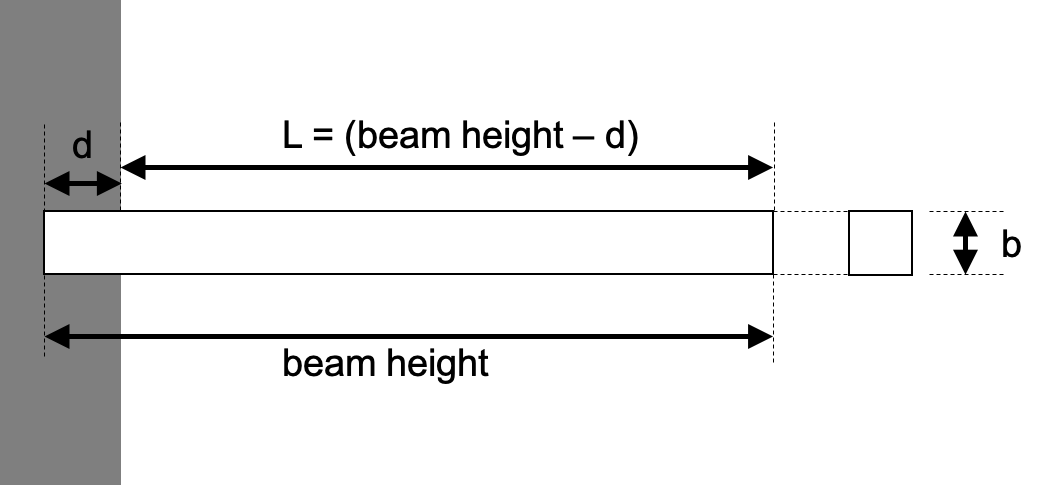
\includegraphics[width=7cm]{cantilever.png}
    % \caption{Parameters of a square beam configured as a cantilever}
    % \label{cantilever}
    % \end{center}
    % \end{figure}
    %}
    
    %\makebox[0pt][l]{%
    \begin{minipage}{\textwidth}
    %\centering
    \begin{center}
    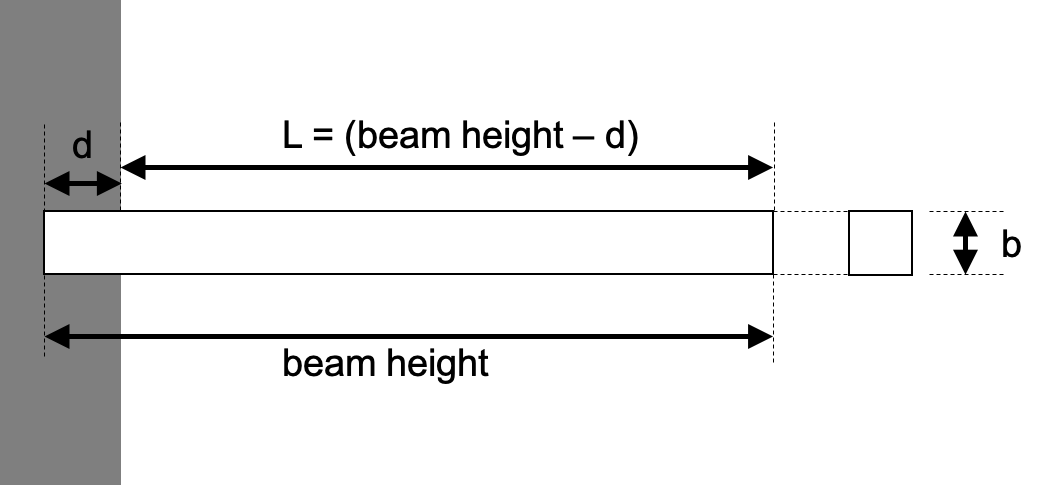
\includegraphics[width=.5\textwidth]{cantilever.png}
    %\caption{Figure 1: }{figure caption}
    \label{fig:fig1}
    \end{center}
    \end{minipage}
    
    \vspace{5mm}
    
    \begin{center}
    \caption{Figure 1: Beam configured as a cantilever showing parameters to calculate bending stiffness}
    \end{center}
    
    \vspace{5mm}
    }
    
    
    Modify your program to:
    \begin{enumerate}[label=(\alph*)]
		\item Use parameters {\tt E} and {\tt BEAMHEIGHT} from the decrypted file to find the bending stiffness in Nmm$^{-1}$ for each beam. Assume the beam is configured as a cantilever where $L = $ ({\tt beam height} - $d$), $d = 10$ cm. {\bf Take care to check the units used in the decrypted file!}
		\item Save the data-set as a .csv file:
		\begin{itemize}
		    \item Include the bending stiffness as an extra column.
		    \item Exclude the {\tt SAMPLE} column from the original data-set.
		\end{itemize} 
	\end{enumerate}
    }

\end{Exercise}

% \begin{Exercise}[title=Importing mulitple files]
% 	\Question{Modify your program so the user now has an additional choice of importing a directory of files in addition to providing an input message and reading a message from a file. Like when importing a file, the program should first check if the directory exists and raise an error of it is not found that prompts the user to enter the name correctly.}
% 	\Question{If the option to import directory is chosen, the program should read in directory, and decrypt/encrypt the contents of each file.}
% 	\Question{Modify the auto-decryption function so that the input from the user to verify if the decryption was successful can be switched on/off using an input argument to the auto-decryption function.}
% 	\Question{Decrypt all files in the folder 'sample_data'. The folder is available on blackbaord. There are 100 files in the folder so turn the user verification off when de-encrypting the files. The files contain the names, customer numbers and number of adult, child and concession tickets for seven different movies. Store the contents of each file as the item of a data structure.}
% \end{Exercise}

% \begin{Exercise}[title=Extracting Information]
% 	\Question{Use the }
% 	\Question{}
% 	\Question{}
% \end{Exercise}

\vspace{1em}
\hrule
\vspace{1em}


\begin{Exercise}[title=(* Optional) Enhancements]

The following section outlines some ideas to extend your program for those students confident with programming and looking to achieve additional marks. \textbf{\underline{This section is optional!}} \newline\textbf{Important:} If you implement any enhancements to your program, you \textbf{must} comment them using the following format:

\vspace{0.5em}
{\tt \#!EXTRA\# Comment here ...}
\vspace{0.5em}

as this will allow the TAs marking your project to easily locate your enhancements. An example comment might start like this:

\vspace{0.5em}
{\tt \#!EXTRA\# Here I create a set of common patterns in English to ...}
\vspace{0.5em}

In the report, discussions related to your enhancements should go in a separate section.\\
\Question{Suggestions for improving the {\tt encrypt} process:
\begin{itemize}
    \item Modify your program so that the user may select {\tt random} instead of a {\tt rotation value}. The cipher will shift the text by a number of places equal to a random number generated by the program.   
    \item Modify the {\tt encryt} process so that for each line in the message, a new rotation value is selected at random, then applied to the line (Update the {\tt decrypt} to decrypt line by line).
\end{itemize}}
\Question{Suggestions for improving the {\tt auto-decrypt} process: 
\begin{itemize}
	\item Modify the program to try every possible rotation value and sort them according to number of words matched with the list of common words. The program should select the solution with the greatest number of instances as the decrypted solution. \newline If the greatest number of instances applies to more than one word, the program should present the solutions to the user to identify which is correct. (This can help reduce how many times you need to ask the user if the rotation is correct.)
% 	This should help reduce how many times you need to ask the user if the rotation is correct.
% 	\item Research and identify common patterns in the English language. Create a function which attempts to match these in the encrypted input message in order to identify the rotation \emph{without} using a common words file.
\end{itemize}}





\end{Exercise}

\vspace{1em}
\hrule
\vspace{1em}

% \subsection*{Helpful hints and suggestions}
% \begin{itemize}
%     \item It is crucial that you complete all of the exercise sheets first - they have been specifically designed to prepare you for this assignment.
% 	\item You should spend plenty of time planning out how the flow of your program might look \textbf{before} you start programming. Look back at previous exercise sheets to see how to approach larger problems by breaking them down into smaller ones.
% 	\item Remember to think about the \textbf{readability} and \textbf{reusability} of your code. Some question you might ask yourself:
% 	\begin{itemize}
% 		\item Have I named things sensibly? Could someone pick up my code and understand it?
% 		\item Am I repeating lots of code? Can I reuse any?
% 		\item Can I simplify the layout of my code to make it more readable? 
% 	\end{itemize}
% 	\item \textbf{Comment your code!} Comments are crucial for many reasons:
% 	\begin{itemize}
% 		\item They help other readers to understand what your code is doing.
% 		\item They help \emph{you} remember what your code is doing, when you come back to it weeks/months/years later. The whole point of writing code is that it can be reused many times, so to make it reusable, add comments.
% 		\item To help your TA assess your understanding of the problem you are trying to solve, and to assess how well your solution solves it. If you use a data structure to implement some functionality, explain it in the comments.
% 	\end{itemize}
% 	Short comments are great to summarise the next several lines of code by giving a high-level overview. For longer, more detailed comments (likely useful in functions and for Part 4), by enclosing them in three speech marks {\tt """} either side. E.g.
	
% 	\vspace{0.5em}
% 	{\tt def SomeFunction(SomeArgument):}\\
% 	{\tt \hspace*{2em}"""}\\
% 	{\tt \hspace*{2em}This function does ...}\\
% 	{\tt \hspace*{2em}....and it does this....}\\
% 	{\tt \hspace*{2em}"""}
% 	\vspace{0.5em}
	
% 	\item We mark for the following points:
% 	\begin{itemize}
% 	    \item Functionality: The more of the functionality described above you implement, the higher the mark.
% 	    \item Types: Proper use of data types and data structures. 
% 	    \item Comments: Appropriate and useful comments. 
% 	    \item Naming: Appropriate variable and function names (remember we want you to use CamelCase)
% 	    \item Report: Informative report, which explains your thought process and analyses the choices you made in your code design. You must reference any external code or ideas used.
% 	    \item Working code: Does the code do what it is supposed to? {\bf READ THE QUESTIONS CAREFULLY to check}. Is the program robust, i.e., does it deal correctly with wrong inputs (user/program interaction).
% 	\end{itemize}
	
% 	\item Finally, don't forget to ask for help! You will be able to ask your TA for help and advice during the weekly drop-in sessions and tutorials. 
% \end{itemize}

\end{document}
